\section{Spheres}
\label{sec:spheres}
In this section we present our $(1+\eps)$-approximation algorithm
for the case of $d$-dimensional spheres.
Let $\C = \{ C_1, C_2, \dots , C_n \}$ be a set of  $n$ number of $d$-dimensional hyperspheres. We denote the radius and profit of each hypersphere \(C_i \in \C\) by \(r_i\) and \(\profit_i\). 
For an object $C_i$ we denote its volume (or area in 2-dimension) to be $\area(C_i)$. 
For a collection of objects $\mathcal{A}$, we define its volume and profit to be $\area(\mathcal{A}):=\sum_{C_i \in A} \area(C_i)$ and $\profit(\mathcal{A}):=\sum_{C_i \in A} \profit(C_i)$, respectively.
We are given a unit knapsack $K := [0,1]^d$. 




We first consider the case of circles, i.e., $d=2$.
Let $\OPT$ be an optimal solution and $\C_{\OPT}$ be the circles in $\OPT$.
Let $\eps \in (0,1/2]$ be a constant and assume that $1/\eps\in\mathbb{N}$. First,
we want to classify the input circles into \emph{small} and \emph{large
}circles such that each large circle is much larger than any small circle.
Due to the following lemma, we can do this such that we can ignore
all circles that are neither large nor small by losing only a factor
of $\eps$. 
We will use this standard shifting argument throughout the paper (see Appendix \ref{sec:shifting} for the details of shifting argumentation). 

%\begin{restatable}
\begin{lem}
%{creategapapx}\emph{($\star$)}
\label{lem:create-gap} Given a constant $\eps\in (0,1)$ and $1/\eps \in \mathbb{N}$, there is a
	set of global constants $\eps^{(0)},...,\eps^{(1/\eps)}\geqslant 0$ such that
	$\eps^{(j)}=(\eps^{(j-1)})^{24}$ for each $j\in\{1,...,{1/\eps}\}$
	and a value $k\in\{1,...,{1/\eps}-1\}$ with the following property: if we define
	$\epsl:=\eps^{(k)}$ and $\epss:=\eps^{(k+1)}$, 
	then sum of profits of all circles $C_i$ in $\OPT$ with radii $\epss \leq r_i \leq \epsl$ is at most $\eps \cdot w(\OPT)$.
\end{lem}
%\end{restatable}
%removed restatable

\begin{proof}
Define $\rho_0=\eps$, and $\rhoi{k} := (\rho_{k-1})^{24}$ for $k \in [1/\eps]$. For each integer $k \in [1/\eps]$,  we define the following sets of items:
$\mathcal{C}_k = \{C_i \in \mathcal{C} \mid r_{i} \in (\rho_{k},\rho_{k-1}]\}$.
Then by pigeonhole principle, one of the sets $\mathcal{C}_{\tau} \cap \OPT$ will contain items of weight at most $\eps w(\OPT)$.
Define $\epsl=\rho_{\tau-1}$ and $\epss=\rho_{\tau}$. The set of $\rho_i$'s defines the set of global constants with cardinality $1/\eps$. 
\end{proof}




We guess the value $k\in\{0,...,1/\eps-1\}$ due to Lemma~\ref{lem:create-gap}.
We define that a circle $C_{i}\in\C$ is \emph{large }if $r_{i}>\epsl$
and \emph{small} if $r_{i}\leqslant\epss$. Also, note that $\epss = \epsl^{24}$. 

\subsection{Guessing large circles} \label{subsec:Large_Guess}

We observe that in $\OPT$ there can be only a constant number of
large circles since each large circle covers a constant fraction of the
available area in the knapsack. 
%\begin{restatable}
\begin{prop}
%{bigsolapx}\emph{($\star$)}
\label{big_sol} Any feasible solution
	can contain at most $(1/\eps)^{O_k(1)}$ large circles. 
	\end{prop}
	%removed restatable
	%\end{restatable}

%\subsection{Proof of \Cref{big_sol}}
\begin{proof}
	Each large circle has area $\pi \epsl^2$. Thus there can be at most $1/(\pi \epsl^2)= 1/(\pi ({\eps^{{24}^k})^2})$ large circles. 
\end{proof}

We guess a feasible solution of the large circles in $\OPT$ that satisfy the packing constraints in time $n^{(1/\eps)^{O_k(1)}}$,
denote them by $\C_{L}^{*}$. In related problems, like the two-dimensional
knapsack problem with squares or rectangles, one can easily guess
the correct placement of the guessed large such objects  
(assuming rational input data).
For packing circles, it is not clear that if there is a packing in which the
centers of the circles are placed at rational coordinates.
% \textcolor{red}
{However, we can still model the circle packing problem as a semi-algebraic set defined via polynomial inequalities, similar to Miyazawa et al.~\cite{MiyazawaPSSW16}.}


We first guess for each circle $C_{i}\in\C_{L}^{*}$
an \emph{estimate }for its placement in $\OPT$. Denote by $\hat{x}_{i}^{(1)},\hat{x}_{i}^{(2)}\in[0,1]$
the coordinates of the center of $C_{i}$ in $\OPT$. We guess values
$\tilde{x}_{i}^{(1)},\tilde{x}_{i}^{(2)}\in\{0,\frac{\eps}{n},\frac{2\eps}{n},...,1\}$
such that $\hat{x}_{i}^{(1)}\in[\tilde{x}_{i}^{(1)},\tilde{x}_{i}^{(1)}+\frac{\eps}{n})$
and $\hat{x}_{i}^{(2)}\in[\tilde{x}_{i}^{(2)},\tilde{x}_{i}^{(2)}+\frac{\eps}{n})$.
Note that there are only $O(n^{2}/\eps^{2})$ possibilities for
each $C_{i}\in\C_{L}^{*}$, and hence only $n^{(1/\eps)^{O_k(1)}}$
possibilities overall for all circles $C_{i}\in\C_{L}^{*}$.

Given these guessed values $\tilde{x}_{i}^{(1)},\tilde{x}_{i}^{(2)}$
for each circle $C_{i}\in\C_{L}^{*}$, we verify that our guess was
correct or not, i.e., confirm that there exists, indeed a corresponding placement
for each circle $C_{i}\in\C_{L}^{*}$ such that the circles in $\C_{L}^{*}$
do not overlap. Therefore, we define a system of quadratic inequalities
 that \agtwo{describes} the problem of finding such a placement.
We require that this placement is consistent with
our guesses $\tilde{x}_{i}^{(1)},\tilde{x}_{i}^{(2)}$ for each $C_{i}\in\C_{L}^{*}$.
\begin{alignat}{2}
\max\{\tilde{x}_{i}^{(1)},r_{i}\}\leqslant x_{i}^{(1)} & \leqslant\min\left\{ \tilde{x}_{i}^{(1)}+\frac{\eps}{n},1-r_{i}\right\}  & \,\,\,\,\, & \forall C_{i}\in\C_{L}^{*}\nonumber \\
\max\{\tilde{x}_{i}^{(2)},r_{i}\}\leqslant x_{i}^{(2)} & \leqslant\min\left\{ \tilde{x}_{i}^{(2)}+\frac{\eps}{n},1-r_{i}\right\}  &  & \forall C_{i}\in\C_{L}^{*}\label{eq:equations}\\
(x_{i}^{(1)}-x_{j}^{(1)})^{2}+(x_{i}^{(2)}-x_{j}^{(2)})^{2} & \geqslant(r_{i}+r_{j})^{2} &  & \forall C_{i},C_{j}\in\C_{L}^{*}\nonumber \\
x_{i}^{(1)},x_{i}^{(2)} & \geqslant0 &  & \forall C_{i}\in\C_{L}^{*}\nonumber
\end{alignat}

Let $|\C_{L}^{*}|=: t$. Then, the above system has $2t$ variables and $k:=O(t^2)$ constraints. 
It is not clear how to compute a solution to this system in polynomial
time. It is not even clear whether it has a solution in which each variable
has a rational value. However, in polynomial time, we can \emph{decide}
whether it has a solution (without computing the solution itself) using an algorithm from \cite{GrigorevVV88}.

Note that the set of solutions satisfying system (\ref{eq:equations}) is a semi-algebraic set in the field of real numbers. 
Thus, whether a given set of circles can be packed or not (the decision problem) reduces to a decision problem of whether
this semi-algebraic set is nonempty or not. 
Here, each constraint $i \in [k]$ in (\ref{eq:equations}) can be written as a function $f_i (x_{1}^{(1)},x_{1}^{(2)}, \dots, x_{t}^{(1)},x_{t}^{(2)})\geqslant 0$ where each $f_i \in \mathbb{Q}[x_{1}^{(1)},x_{1}^{(2)}, \dots, x_{t}^{(1)},x_{t}^{(2)}]$ is a polynomial with rational coefficients of degree at most two.
Therefore, deciding the circle packing problem is equivalent to deciding whether the following formula is satisfiable or not: $F:= (\exists x_{1}^{(1)})(\exists x_{1}^{(2)}) \dots (\exists x_{t}^{(1)}) (\exists x_{t}^{(2)}) \land_{i=0}^{k} f_i(x_{1}^{(1)},x_{1}^{(2)}, \dots, x_{t}^{(1)},x_{t}^{(2)}) \geqslant 0$. 
To solve this decision problem, we use the following result.

\begin{theorem}[\cite{GrigorevVV88}]
	\label{thm:GrigorevVV88}
	Let $f_1, f_2, \dots, f_k \in \mathbb{Q}[x_{1}^{(1)},x_{1}^{(2)}, \dots, x_{t}^{(1)},x_{t}^{(2)}]$ be polynomials with absolute value of any coefficient to be represented by $M$ bits and maximum degree $\Delta$.
	There is an algorithm that decides whether the formula $F:= (\exists x_{1}^{(1)})(\exists x_{1}^{(2)}) \dots (\exists x_{t}^{(1)}) (\exists x_{t}^{(2)}) \land_{i=0}^{k} f_i(x_1, y_1, \dots, x_n, y_n) \geqslant 0$ is true, with a running time of $M^{O(1)}(k\Delta)^{O(t^2)}$.
	
	If it is true, the algorithm also returns polynomials $f, g_1, h_1, \dots, g_t, h_t \in \mathbb{Q}[x]$ with coefficients of bit size at most $M^{O(1)} (k \Delta)^{O(t)}$ and maximum degree $k^{O(t)}$, such that for a root $x$ of $f(x)$, the assignment $x_{1}^{(1)}=g_1(x), x_{1}^{(2)}=h_1(x), \dots, x_{t}^{(1)}=g_n(x), x_{t}^{(2)}=h_n(x)$
	satisfies the
	formula $F$.
	
	Moreover, for any rational $\alpha>0$, it returns values $\bar{x}_{1}^{(1)},\bar{x}_{1}^{(2)} \dots, \bar{x}_{t}^{(1)},\bar{x}_{t}^{(2)} \in \mathbb{Q}$ such that $| \bar{x}_{i}^{(1)}- {x}_{i}^{(1)} | \leqslant \alpha$ and  $| \bar{x}_{i}^{(2)}- {x}_{i}^{(2)} | \leqslant \alpha$, for $1 \leqslant i \leqslant t$, in time at most $(\log (1/\alpha) M)^{O(1)} (k \Delta)^{O(t^2)}$.
\end{theorem}




We crucially use here that our system has only constantly many variables
and constraints,~i.e., in (\ref{eq:equations}), we have that $\Delta, k, t$ are constants and that $M$ is polynomially bounded in $n$.
From \Cref{thm:GrigorevVV88}, we see that
in polynomial time we can decide whether
(\ref{eq:equations}) has a solution.

If the system (\ref{eq:equations}) does
not have a solution, then we reject this guessed combination of $\C_{L}^{*}$
and values $\tilde{x}_{i}^{(1)},\tilde{x}_{i}^{(2)}$ for each circle
$C_{i}\in\C_{L}^{*}$. We assume in the following that it has a solution.
Observe that the guessed values $\tilde{x}_{i}^{(1)},\tilde{x}_{i}^{(2)}$
yield an estimate for $\hat{x}_{i}^{(1)},\hat{x}_{i}^{(2)}$ up to
a (polynomially small) error of $\eps/n$.

Now we will improve this even to an \emph{exponentially} small error of $1/2^{n/\eps}$.


\subsubsection{Improving the precision of the large spheres}
\label{subsec:Improve_Large} Recall that for each large circle $C_{i}\in\C_{L}^{*}$
we guessed its center in the optimal packing up to a polynomial error
of $\frac{\eps}{n}$. We improve this to only an exponential error
of at most $\frac{1}{2^{n/\eps}}$. To do this, we apply Theorem~\ref{thm:GrigorevVV88}
with $\alpha:=\Theta(\frac{1}{2^{n/\eps}})$. This yields more precise
estimates $\bar{x}_{i}^{(1)},\bar{x}_{i}^{(2)}$ for each $C_{i}\in\C_{L}^{*}$.
There is an important subtlety though: for our guessed coordinates
$\tilde{x}_{i}^{(1)},\tilde{x}_{i}^{(2)}$ we can assume that they
differ from the coordinates of $\OPT$ by at most our polynomial error
of $\frac{\eps}{n}$. For the new estimates $\bar{x}_{i}^{(1)},\bar{x}_{i}^{(2)}$
we can \emph{not }guarantee this: our subroutine from Theorem~\ref{thm:GrigorevVV88}
possibly returns a solution that is (close to) feasible for the
large circles, but not (close to) a solution that is feasible for
the large and for the small circles. Because of this, we guessed the estimates
$\tilde{x}_{i}^{(1)},\tilde{x}_{i}^{(2)}$ for each $C_{i}\in\C_{L}^{*}$,
so that we can assume that these estimates really correspond to $\OPT$
and not just to some arbitrary solution to \eqref{eq:equations}.

If it were true that there is always a $(1+\eps)$-approximate solution
in which the center of each circle has rational coordinates that can
be encoded with a polynomially bounded number of bits, then we could
choose $\alpha$ appropriately to compute it. More precisely, we could
compute a range for each coordinate that contains only one rational
number with a bounded number of bits, and we could compute this number
afterward.


\subsection{Placing small circles}\label{subsec:placing_small}

We want to select small circles from $\C$ and place them inside the
knapsack, so that they do not overlap with each other or
with the circles in $\C_{L}^{*}$. To this end, we define $\epsc := \epsl^{12}$ (i.e., $\epss=\epsl^{12} \epsc = \epsc^2)$ to subdivide the knapsack
into a grid with $1/\epsc^2$ square grid cells of side length $\epsc$ . Our choice of parameters ensures that each small circle is small compared to each grid
cell and each large circle is big compared to each grid cell. Formally, for each $\ell,\ell'\in\{0,1, \dots ,\frac{1}{\epsc}-1\}$
we define a grid cell $G_{\ell,\ell'}:=[\ell\cdot\epsc,(\ell+1)\cdot\epsc)\times[\ell'\cdot\epsc,(\ell'+1)\cdot\epsc)$.
We define the set of all grid cells by $\G:=\{G_{\ell,\ell'}:\ell,\ell'\in\{0,1, \dots ,1/\epsc-1\}\}$.

We say that a placement of a circle $C_{i}\in\C_{L}^{*}$ is \emph{legal} if its
center is placed at a point $(x_{i}^{(1)},x_{i}^{(2)})$ such that
$\max\{\tilde{x}_{i}^{(s)},r_{i}\}\leqslant x_{i}^{(s)}\leqslant\min\left\{ \tilde{x}_{i}^{(s)}+\frac{\eps}{n},1-r_{i}\right\} $
for each $s\in\{1,2\}$. We show that there is a structured packing with near-optimal profit in which each small circle is contained in a grid cell
that does not intersect with any large circle in $\C_{L}^{*}$ in any legal packing of them. This will allow us to decouple the remaining problem
for the small circles from the large circles, even though we do not know the exact placement for the latter.
Moreover, in each grid cell the small circles use only a reduced area of size $(1-\eps) \epsc \times(1-\eps) \epsc$.
Let $\C_{S}^{*}$ denote the small circles in $\OPT$.

\begin{lemma}\label{lem:structured-packing}
	In polynomial time, we can compute a set of grid cells $\G_w$ such that no grid cell in $\G_w$ intersects with any
	circle $C_i \in\C_{L}^{*}$ for any legal placement of $C_i$. Moreover, there is a set of small circles $\C_S \subseteq \C_{S}^{*}$ such that $w(\C_{S}) \geqslant (1-\eps)w(\C_{S}^{*})$ and
	the circles in $\C_S$ can be packed non-overlappingly inside $|\G_w|$ grid cells of size $(1-\eps) \epsc \times(1-\eps) \epsc$ each.
\end{lemma}
We will prove Lemma~\ref{lem:structured-packing} later in Section~\ref{sec:structured-packing}. Using it, we compute an approximation to the set $\C_S$ via \ari{\Cref{cor:fat-ra}.}


We pack the computed circles into our grid cells $\G_w$, and denote them by $\C'_S$. In particular, they do not intersect any of the
large circles in $\C_{L}^{*}$ in any legal placement of them. Our solution (corresponding to the considered guesses) consists of $\C_{L}^{*}\cup \C'_S$. Recall that we can guarantee that these circles can be packed non-overlappingly inside the knapsack. Also, for the circles in
$\C'_S$ we computed their placement \emph{exactly} and for the circles in $\C_{L}^{*}$ we computed their placement up to our polynomially small error of $\eps/n$. As mentioned in Section~\ref{subsec:Improve_Large}, we can then reduce this error to an exponentially small error.

\subsection{Structural packing for small circles}\label{sec:structured-packing}
In this section, we prove Lemma~\ref{lem:structured-packing}.
First, we show that intuitively almost \agtwo{every} small circle in $\C_{S}^{*}$ is contained inside some grid cell.
Formally, we show that the total area of all other small circles in $\C_{S}^{*}$ is small.
For any set $\mathcal{S}$ of circles or grid cells, we define $a(\mathcal{S})$ to be the total area of the elements in $\mathcal{S}$.

%\begin{restatable}
\begin{lem}
%{smallcirclesgridcellslemmaapx}\emph{($\star$)}
	\label{lem:small-circles-grid-cells}
	Let $\mathcal{C}_{cut}\subseteq \C_{S}^{*}$ be the set of all small circles in $\C_{S}^{*}$ that intersect more than one grid cell. We have that $\area(\mathcal{C}_{cut}) \leqslant 8 \epss/\epsc \leqslant \eps \epsl^2/64$.
\end{lem}
%\end{restatable}

	
\begin{proof}
Each small circle has diameter at most $2\epss$. 
	For each horizontal (resp. vertical) gridline $\ell$, each $C \in \mathcal{C}_{cut}$ must lie in a strip of height (resp. width) $4\epss$ and width (resp. height) 1. Totally there are $2/\epsc$ gridlines (see Figure~\ref{fig:cut_cell_illustration}).
    
    \begin{figure}[h!]
	\begin{center}
		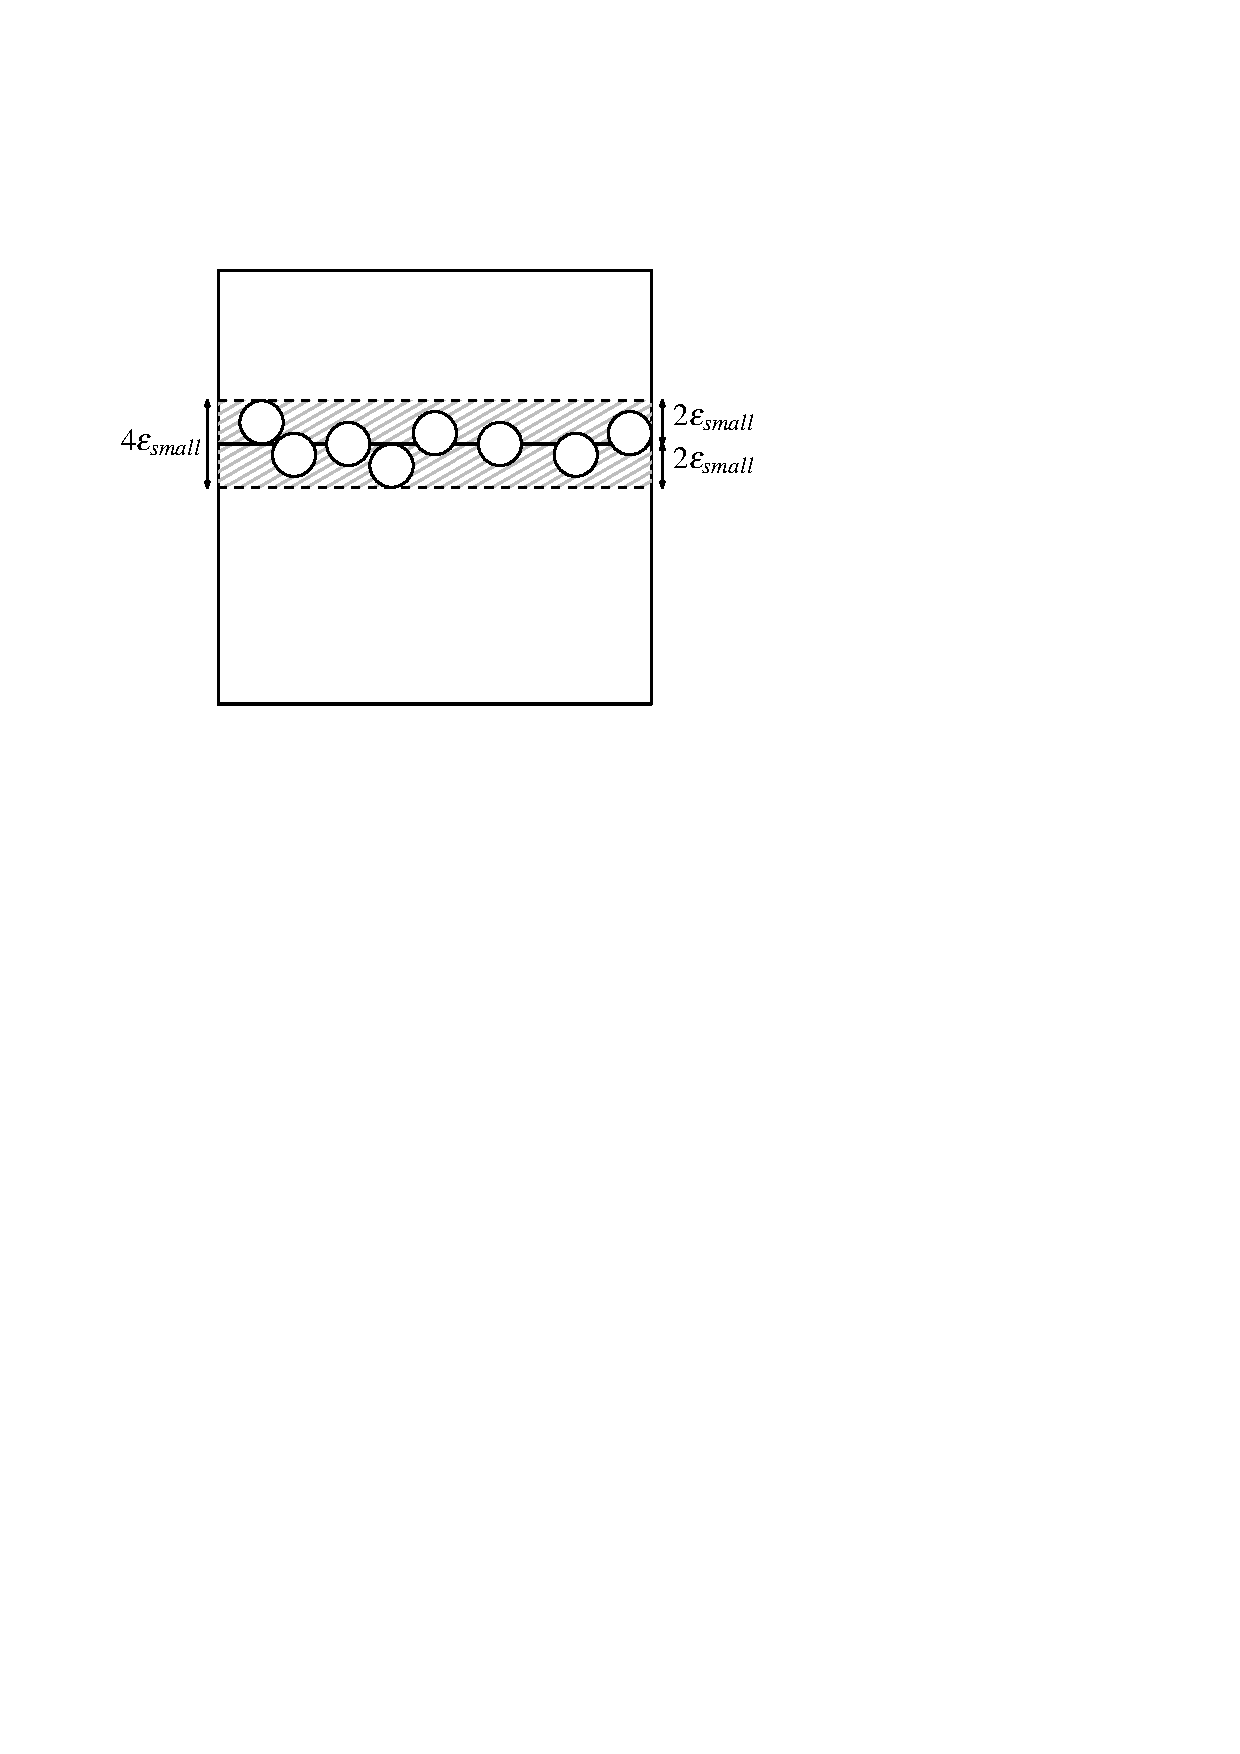
\includegraphics[width=9cm]{Figures/line631-632.pdf}
		\caption{Obtaining the strip of height \(4\eps_{small}.\)}
		\label{fig:cut_cell_illustration}
	\end{center}
    \end{figure}
 
	Thus $\area(\mathcal{C}_{cut}) \leqslant 8 \epss/\epsc = 8 \epsl^{12}  \leqslant  \eps \epsl^2/64$. The last inequality follows from the fact that $\epsl \leqslant \eps \leqslant 1/2$.
\end{proof}




We will repack the circles in $\mathcal{C}_{cut}$ later such that each of them is contained inside one single grid cell.
Thus, for each small circle $C_{i}\in\C_{\OPT} \setminus \C_{cut}$ there is a grid cell $G_{\ell,\ell'}$ for
some $\ell,\ell' \in\{0,1,...,1/\epsc-1\}$ such that $C_{i}$ is contained in $G_{\ell,\ell'}$ in $\OPT$.
When we select and place small circles, we must be careful
that they do not intersect any large circles from $\C_{L}^{*}$. One
difficulty for this is that we do not know the precise coordinates
of the large circles. Therefore, we place small circles only into grid
cells that do not overlap with any large circle from $\C_{L}^{*}$ in
any legal placement of them.
Formally, we partition the cells
in $\G$ into three types: white, gray\label{key}, and black cells (see \Cref{fig:grid_cell_partition}).
\begin{figure}[h]
		\begin{center}
		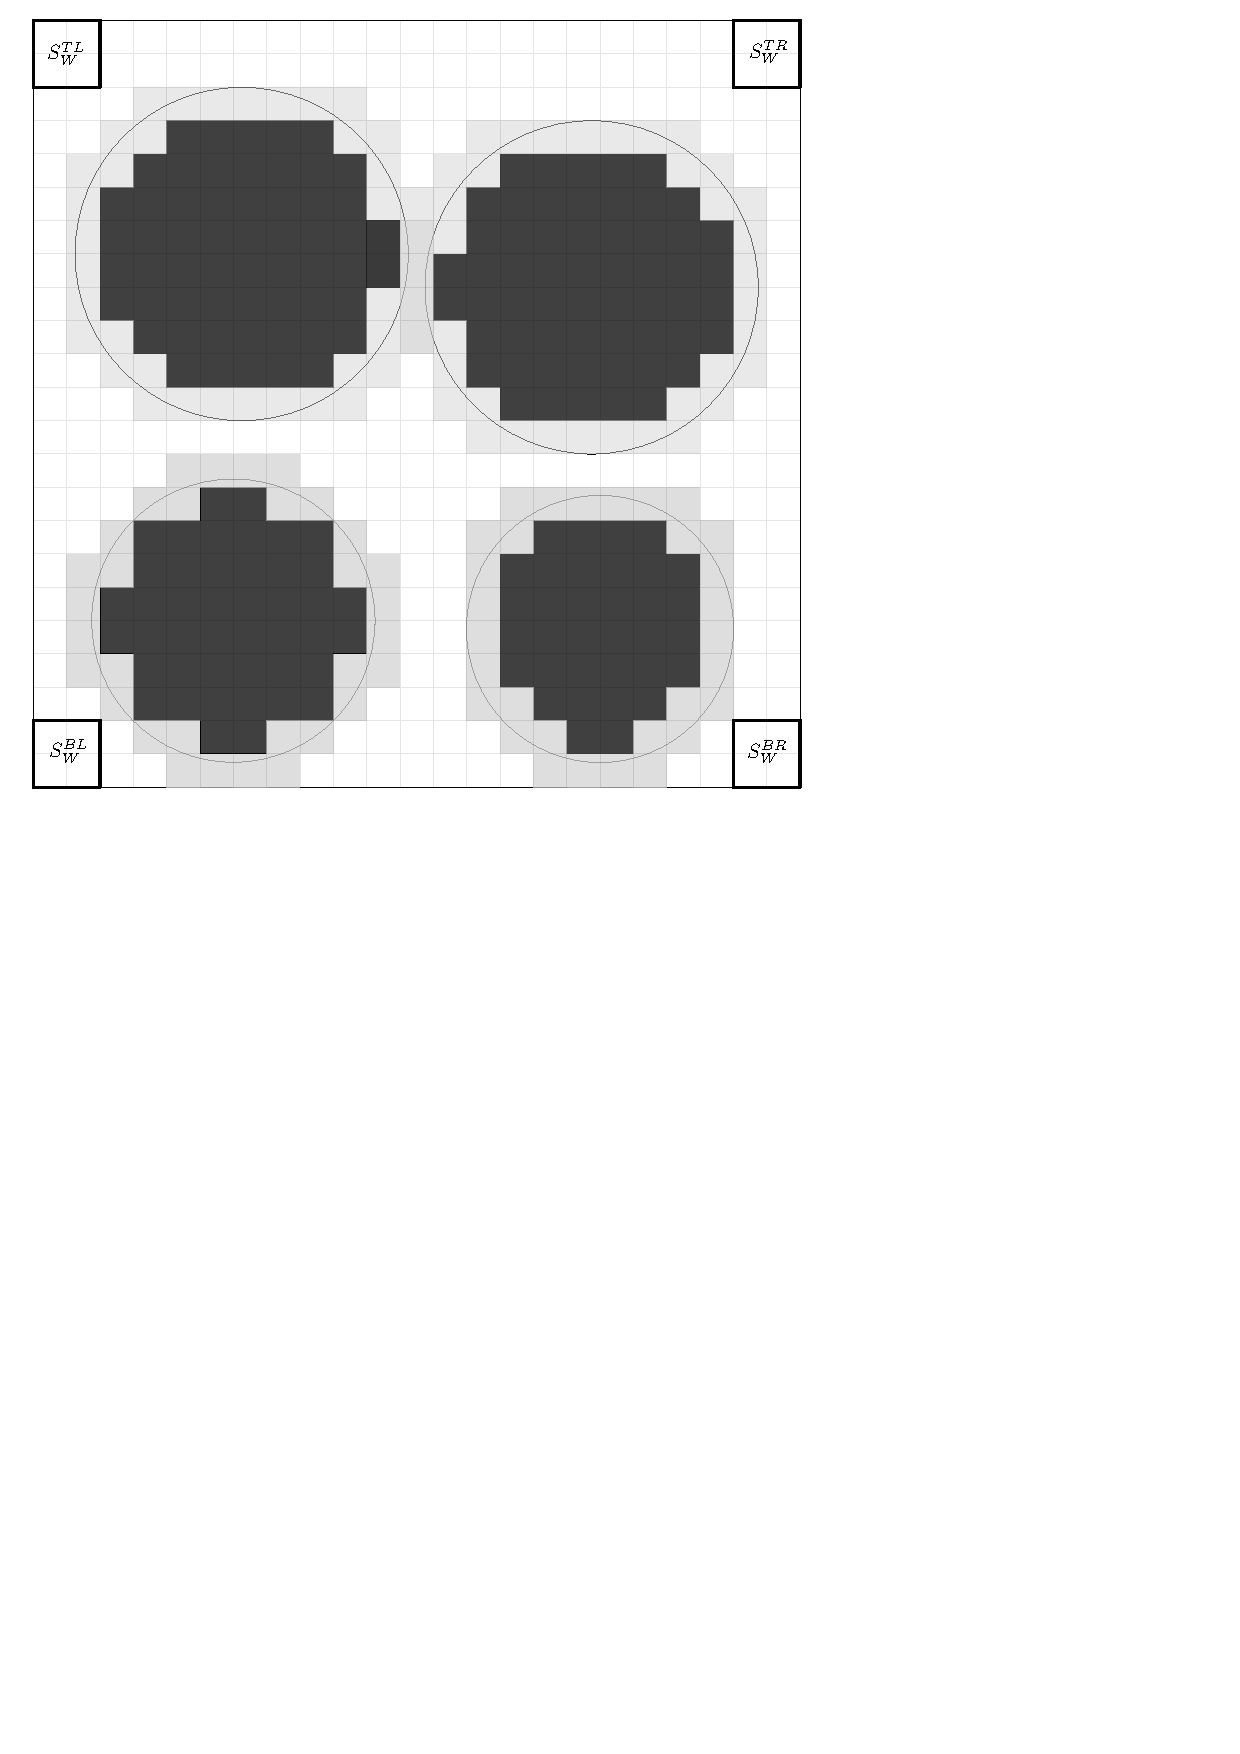
\includegraphics[width=8cm]{Figures/email-figure-1-final.pdf}
		\caption{Partitioning grid cells into white, black, and gray cells. Later corner regions $S_W^{BL}, S_W^{TL}, S_W^{BR}, S_W^{TR}$ are used to to pack items in gray cells. }
		\label{fig:grid_cell_partition}
	\end{center}
\end{figure}
\begin{defn} Let $G_{\ell,\ell'}\in\G$ for some $\ell,\ell'\in\{0,1,...,1/\epsc-1\}$.
	The cell $G_{\ell,\ell'}$ is
	\begin{itemize}
		\item \emph{white} if $G_{\ell,\ell'}$ does not intersect with any circle
		$C_{i}\in\C_{L}^{*}$ for any legal placement of $C_{i}$,
		\item \emph{black} if $G_{\ell,\ell'}$ is contained in some circle $C_{i}\in\C_{L}^{*}$
		for any legal placement of $C_{i}$,
		\item \emph{gray }if $G_{\ell,\ell'}$ is neither white nor black.
	\end{itemize}
	
	
\end{defn} The gray cells are problematic for us since a gray cell
might be (partially) covered by a large circle in $\C_{L}^{*}$ but
we do not know by how much (and which part of the cell). Therefore,
we do not place any small circles into gray cells. However, $\OPT$
might place small circles into these cells (and obtain the profit of
these circles). On the other hand, we can show that the number of gray
cells is very small, only a small fraction of all grid
cells can be gray. In order to do this, we use \agtwo{the fact} that the values $\tilde{x}_{i}^{(1)},\tilde{x}_{i}^{(2)}$
for each circle $C_{i}\in\C_{L}^{*}$ estimate the placement of each
large circle relatively accurately, and that the grid cells are relatively
small. This allows us to prove that almost all
cells are black or white. Also, we can compute all gray
cells efficiently. Let $\G_{g}\subseteq\G$ denote
the set of all gray grid cells in $\G$. 


%\begin{restatable}
\begin{lem}
%{graycircleslemmaapx}\emph{($\star$)}
	\label{lem:gray-circles}
	The total area of gray cells $\area(\G_{g})$ is at most $\eps \epsl^2/5$. We can compute $\G_g$ in polynomial time.
\end{lem}
%{restatable}
%\subsection{Proof of \Cref{lem:gray-circles}}

\begin{figure}[ht]
	\begin{center}
		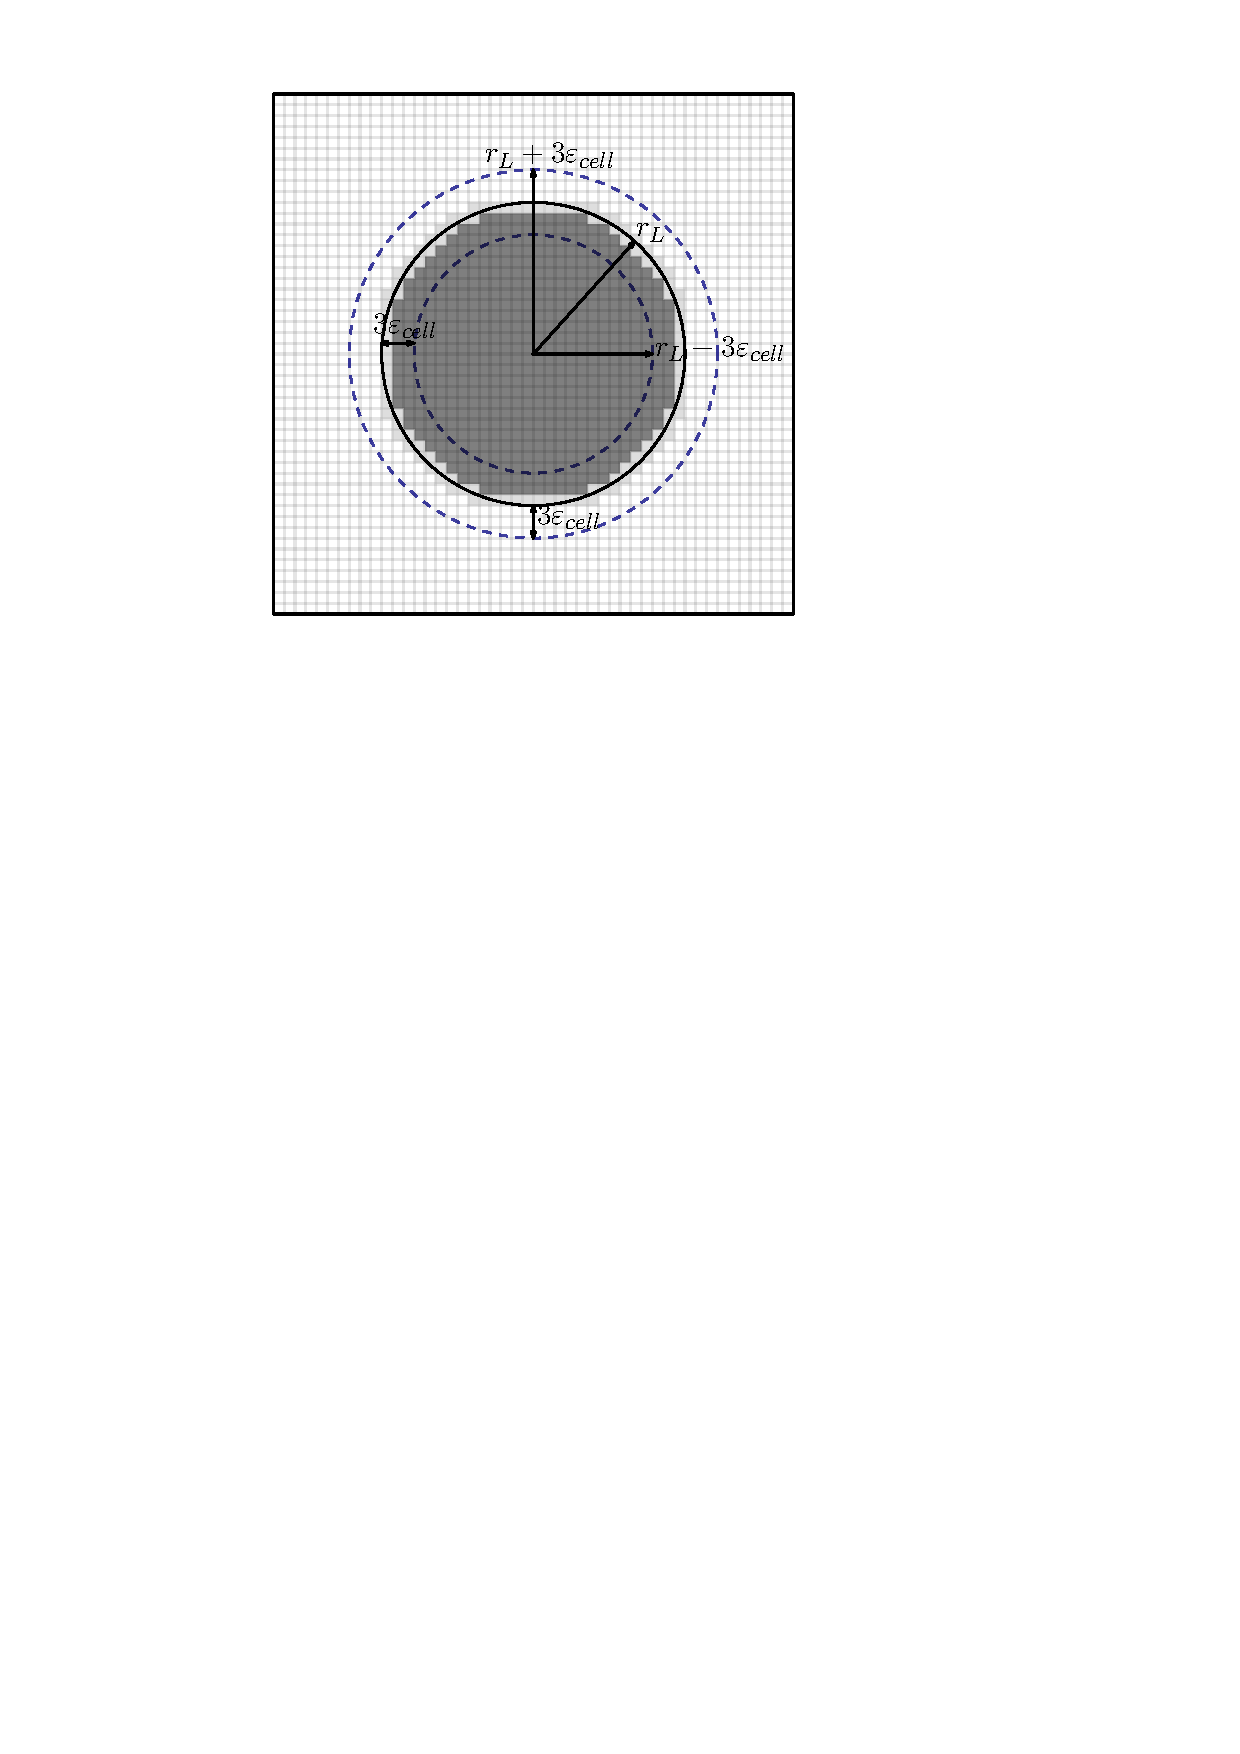
\includegraphics[width=8cm]{Figures/gray_white_black_cells_illustration.pdf}
		\caption{Three types of cells for a particular circle}
		\label{fig:gray_cell_partition_types}
	\end{center}
\end{figure}
\begin{proof}
	Consider a large circle $C_L$ with radius $r_L \geqslant \epsl$. Let $\G_{g, C_L}, \G_{b, C_L}$ be the set of gray and black grid cells that overlap with $C_L$.
	We will first show that $\G_{g, C_L}$ is much smaller compared to  $\G_{b, C_L}$.
	Note that for $C_L$,  we only have an estimate $\tilde{x}_{C}^{(1)},\tilde{x}_{C}^{(2)}$ of the coordinate of its center up to
	a \emph{polynomially} small error of $\eps/n$. 
	
	First, we claim that all the cells intersected by a circle centered at  $(\tilde{x}_{C}^{(1)},\tilde{x}_{C}^{(2)})$ of radius $r_L- 3\epsc$ are in $\G_{b, C_L}$. 
	For contradiction, assume there is a gray cell $S_g$ intersected by a circle $C$ centered at  $(\tilde{x}_{C}^{(1)},\tilde{x}_{C}^{(2)})$ of radius $r_L- 3\epsc$.
	Then, the distance of any point in $S_g$ from the center of the circle is at most $r_L- 3\epsc +\sqrt{2}\epsc < r_L-\eps/n$ for large enough $n$. Thus  $S_g$  is completely contained within $C$.
	
	Similarly, we can show that the cells that are outside of a circle centered at  $(\tilde{x}_{C}^{(1)},\tilde{x}_{C}^{2})$ of radius $r_L+ 3\epsc$ are not in $\G_{b, C_L}$.
	
	Hence, $\area(\G_{b, C_L}) \geqslant \pi (r_L- 3\epsc)^2$ and $\area(\G_{g, C_L}) \leqslant \pi (r_L+3\epsc)^2 - \pi(r_L-3\epsc)^2=12 \pi \epsc r_L$.
	Hence, 
	\[
	\frac{\area(\G_{g, C_L})}{\area(\G_{b, C_L})} \leqslant \frac{12 \pi \epsc r_L}{\pi (r_L- 3\epsc)^2} \leqslant \frac{12 \epsc r_L}{(r_L/2)^2} \leqslant 48\frac{\epsc}{\epsl} = 48 \epsl^{11} \leqslant \eps \epsl^2/5
	\]
	The second inequality follows from the fact that $\epsl \leqslant \eps \leqslant 1/2$ and $r_L \geqslant \epsl$.  The last inequality uses the fact that $\eps \leqslant 1/2$.
	Therefore, $\sum_{C \in \C_{L}^{*}} {\area(\G_{g, C_L})} \leqslant (\eps \epsl^2/5) \cdot \sum_{C \in \C_{L}^{*}}  {\area(\G_{b, C_L})} \leqslant \eps \epsl^2/5$.
\end{proof}

See Figure~\ref{fig:gray_cell_partition_types} for an illustration. 

Unfortunately, it is not sufficient for us that there are
only a few gray cells. It might be that almost all cells are either
gray or black and, hence, we need to place most of the selected small
circles into gray cells (in order to obtain an $(1+\eps)$-approximate
solution).

However, we can show that this is not the case. We prove that the
number of white cells (which we can safely use for small circles) is
at least by a factor $1/\eps$ larger than the number of gray
cells. To show this, we exploit the geometry of the circles. In each
corner of the knapsack, there are cells that cannot intersect with
any large circle, simply because the grid cells are small compared to
the large circles and because of the shape of the large circles (see the corner regions in \Cref{fig:grid_cell_partition}).
Hence, these grid cells are white. Let $\G_{w}\subseteq\G$ denote
the set of all white grid cells in $\G$. 

%\begin{restatable}
\begin{lem}
%{whitecircleslemmaspx}\emph{($\star$)}
	\label{lem:white-circles}
	The total area of white grid cells $\area(\G_{w})$ is at least $\epsl^2/4$. We can compute $\G_w$ in polynomial time.
\end{lem}
%restatable}
%\subsection{Proof of \Cref{lem:white-circles}}
\begin{figure}[ht]
	\begin{center}
		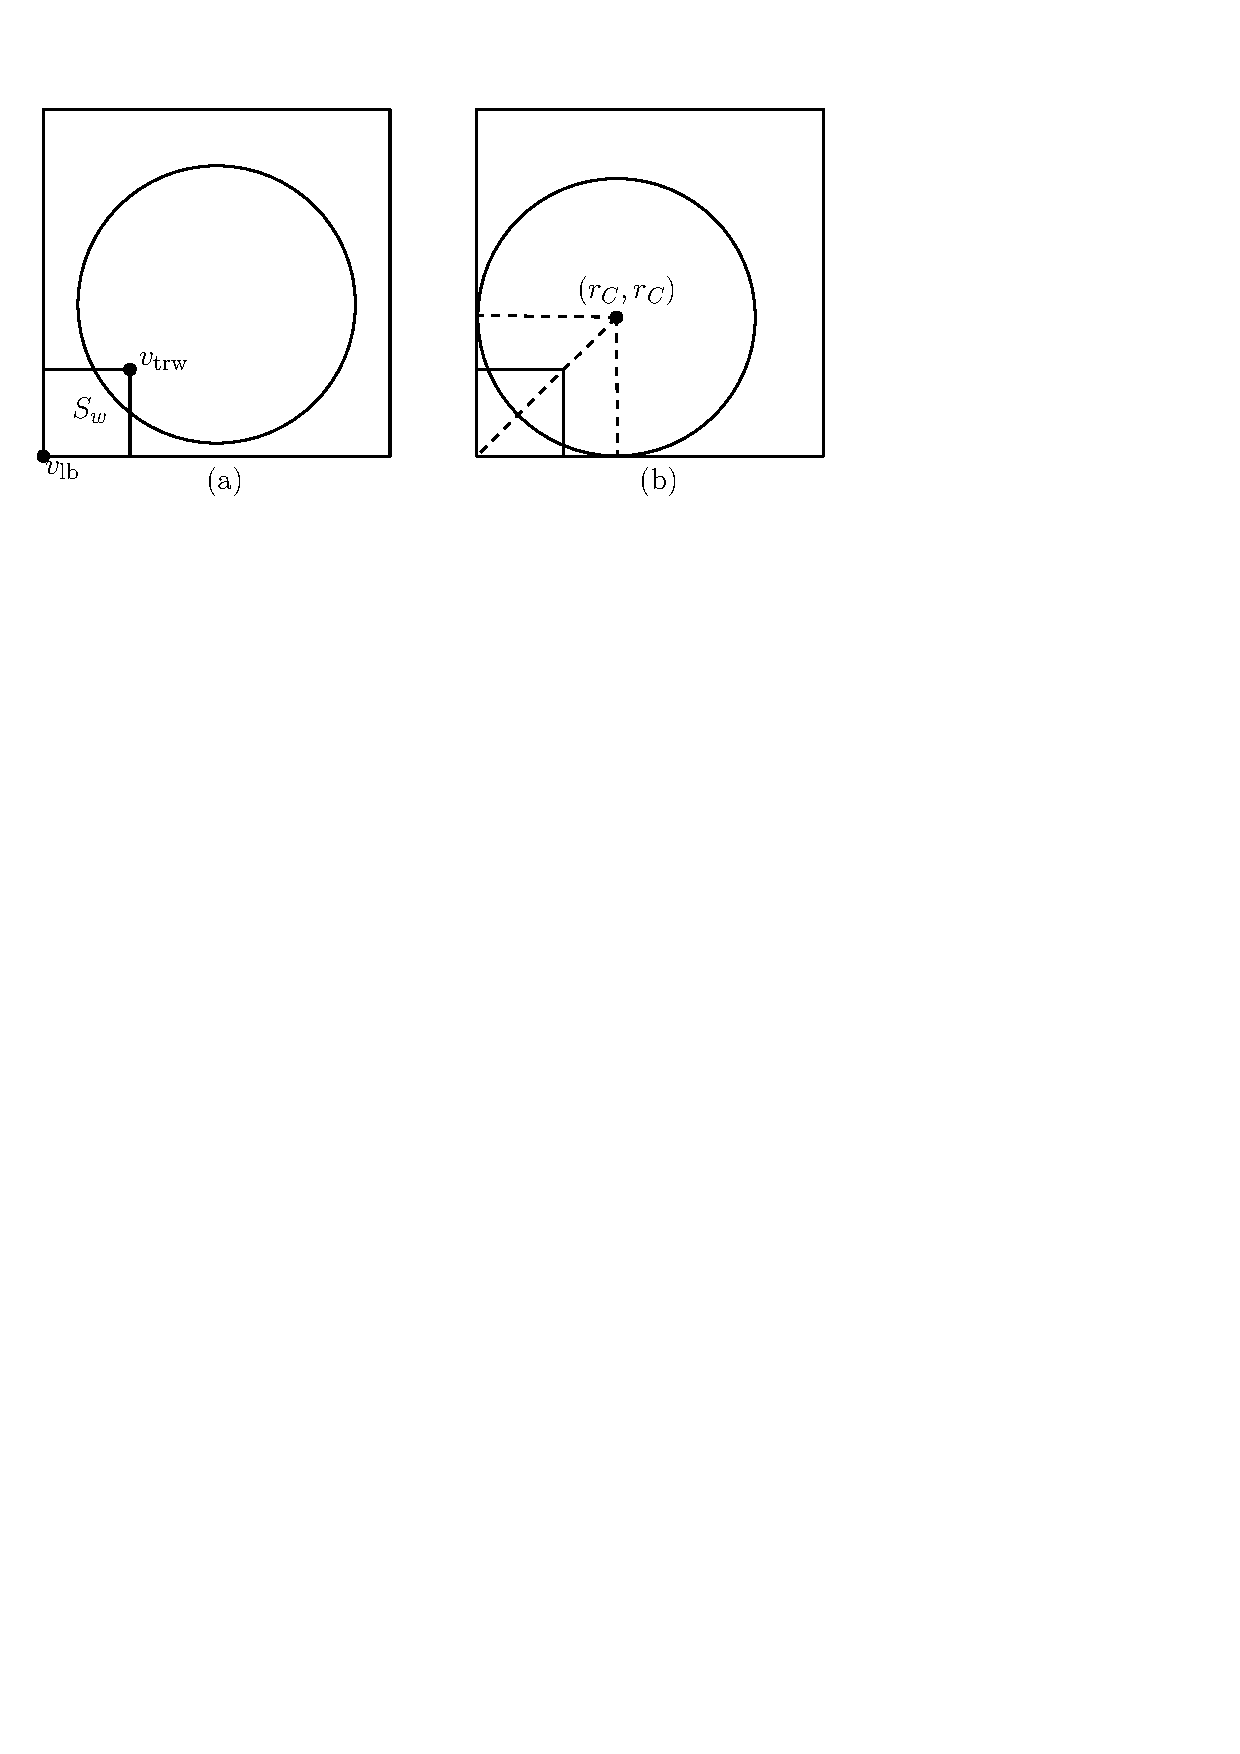
\includegraphics[width=8cm]{Figures/email-figure-2-3.pdf}
		\caption{(a) The square \(S_w\) and the large circle \(C\), (b) Orientation of circle \(C\) after translation}
		\label{fig:corner_cell}
	\end{center}
\end{figure}

\begin{proof}
	In \Cref{fig:corner_cell}, consider a corner (w.l.o.g., left bottom corner) $v_{lb}$ of the knapsack. Let  $S_w$ be a square region of side length $\epsl/2$ such that $S_w$ is contained in the knapsack and shares $v_{lb}$.
	We will show that no large circles intersect $S_w$ and thus all grid cells in $S_w$ are white.
	
	For contradiction, assume that some large circle $C$ intersects $S_w$. As $r_C \geqslant \epsl$, if $C$ intersects either the top or right edge of $S_w$ it must contain the top right corner of $S_w$ at $(\epsl/2, \epsl/2)$.  Thus, $(\epsl/2, \epsl/2)=: v_{trw} \in interior(C)$. 
	Then consider $C$ in the knapsack and we can move $C$ towards $v_{lb}$  such that it touches two boundary edges of the knapsack, i.e.,  the center of $C$ is now at $(r_C, r_C)$. Note that, after this translation, $C$ should continue to intersect $S_w$, i.e.,  $(\epsl/2, \epsl/2) \in interior(C)$. 
	However, distance of $v_{trw}$ from $(r_C, r_C)$ is $\sqrt{(r_C-\frac{\epsl}{2})^2 + (r_C-\frac{\epsl}{2})^2} \geqslant \sqrt{2(\epsl-\frac{\epsl}{2})^2} \ge \epsl$.
	Thus,  $v_{trw} \notin interior(C)$. This is a contradiction. 
	
	We argue this analogously for all the corners of the knapsack to complete the proof. 
\end{proof}


Using Lemmas \ref{lem:small-circles-grid-cells}, \ref{lem:gray-circles},
and \ref{lem:white-circles}, we show that there is a $(1+\eps)$-approximate
solution in which each small circle is contained in some white cell;
in particular, no small circle is placed inside a gray cell. To prove
this, we delete all small circles in the $O(\eps |\G_w|)$ white grid
cells with the smallest total profit among all white cells and place all circles from gray cells and
all circles from $\C_{cut}$ into those.

%\begin{restatable}[$\star$]
\begin{lem}%{smallcircleswhitegridcellslemmaapx}
	\label{lem:small-circles-white-grid-cells-1}
	There is a set $\C'_S \subseteq \C^*_S$ of small circles with $p(\C'_S)\geqslant (1-O(\eps)) p(\C^*_S)$ such that there is a packing for $\C'_S$ using the grid cells in $\G_w$ only.
	\end{lem}
%\end{restatable}

\begin{proof}
	We delete all circles in the $2\eps$ fraction of white cells with the smallest total
	weight among all white cells, incurring an $2\eps$ fraction loss in the weight.
	This makes $\eps \epsl^2/2$ space available for packing circles in the gray cells and $\C_{cut}$.
	Now, the total volume of circles in the gray cells and $\C_{cut}$ is at most  $\eps \epsl^2/5 + \eps \epsl^2/64 \leqslant \eps \epsl^2/4$. As these circles are small, the available space is enough to pack them even using the \texttt{NFDH} algorithm. 

	Recall that the radius of each
	small circle is at most $\epss$, which is at least by a factor
	$1/\eps$ smaller than the size of each grid cell (which is $\epsc \times\epsc$).
	Therefore, with a shifting argument, we can show that from each grid
	cell $G_{\ell,\ell'}\in\G$ we can delete small circles from $\C^*_S$ contained in
	$G_{\ell,\ell'}$ whose total profit is only an $O(\eps)$-fraction
	of the overall profit of those circles, such
	that the remaining circles in $G_{\ell,\ell'}$ fit even inside a smaller
	grid cell of size $(1-\eps)\epsc \times(1-\eps)\epsc$.
	If we apply this operation to each grid cell in $\G_{w}$, the remaining
	circles fit non-overlappingly into $|\G_{w}|$ (small) knapsacks of
	size $(1-\eps)\epsc \times(1-\eps)\epsc$
	each.
\end{proof}

We complete the proof of Lemma~\ref{lem:structured-packing} by applying the following lemma to $\C_{S}:= \C''_{S}$
which shows that we can sacrifice a factor of $1+O(\eps)$ \agtwo{to be} able to use resource augmentation when we pack the small circles.

%\begin{restatable}[$\star$]{lem}{gridresourceaugmentationlemmaapx}
\begin{lem}
	\label{lem:grid-resource-augmentation-1}
	There is a set of small circles $\C''_{S}\subseteq\C'_{S}$ such that $w(\C''_{S})\ge(1-\eps)w(\C'_{S})$ and it is possible to place the circles in $\C''_{\sml}$ non-overlappingly inside $|\G_{w}|$ square knapsacks of size $(1-\eps)\epsc \times(1-\eps)\epsc$ each.
	\end{lem}

\begin{proof}
	Consider a square knapsack in $\G_{w}$ of side length $\epsc$.
        Consider a random strip $[x, \min\{\epsc, x+\eps\epsc\}]\times [0,\epsc] \cup [0, \max\{0, x+\eps\epsc -\epsc\}] \times [0,\epsc]$ of width $\eps\epsc$ where $x$ is chosen uniformly at random in $[0,\epsc]$. Then the probability of a small circle of radius $r$ intersected by the strip is at most $(2r+\eps\epsc)/\epsc$.
	By removing all circles intersected by a random strip of height (resp. width) $\epsc$ and width (resp. height) $\eps\cdot\epsc$ in both directions, we incur a loss of at most $2(2 r/\epsc + \eps)$ fraction of optimal profit. As $r\le \epss$, we incur a loss of at most $O(\eps)$ fraction of profit as $\epss = \epsc^2 = \epsl^{24}$.
\end{proof}



\subsection{Higher dimensions}

Our techniques from the previous section extend directly to the problem of packing
hyperspheres in any (constant) dimension $d$ which yields our main theorem for the setting of packing
(hyper-)spheres. See Appendix for the detailed proof. 

\begin{theorem}\label{thm:d-dim-ptas} Let $d\in\N$ be a fixed constant. For the geometric knapsack problem with
	$d$-dimensional hyperspheres, there is a polynomial time algorithm
	that computes a set of hyperspheres $\tilde{\C}$ with $p(\tilde{\C})\geqslant(1-\eps)\OPT$
	that can be placed non-overlappingly inside the knapsack. For all
	but $O_{\eps}(1)$ hyperspheres in $\tilde{\C}$ we compute the
	precise coordinate of the corresponding packing; for the other $O_{\eps}(1)$
	circles we compute an estimate of the packing with an additive error
	of at most $\frac{1}{2^{n/\eps}}$ in each dimension. \end{theorem}

